\documentclass{article}

\usepackage{tikz}
\usetikzlibrary{quotes,shapes.multipart,positioning,matrix,calc}

\usepackage{minted}
\usepackage{booktabs}

\usepackage{enumitem}
\setlist[enumerate, 1]{label=(\alph*)}
\setlist[enumerate, 2]{label=\roman*.}

\usepackage{titlesec}

\titlelabel{Question \thesection: }

\title{
    15-415/615 - Database Applications

    Answers to Homework 4
}
\author{Shangning Xu}

\begin{document}

\maketitle

\newpage

\section{ISAM}

\begin{enumerate}
    \item \begin{enumerate}
        \item 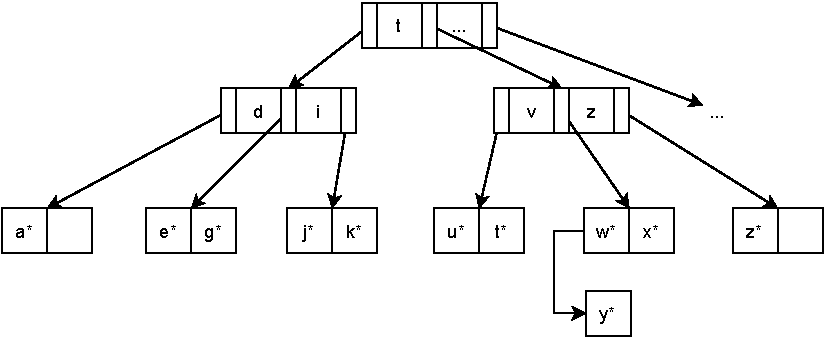
\includegraphics[width=\linewidth]{img/4-1-a-i.pdf}
        \item 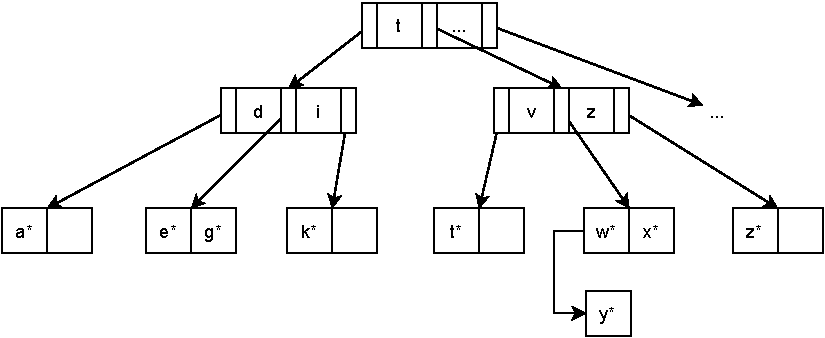
\includegraphics[width=\linewidth]{img/4-1-a-ii.pdf}
        \item 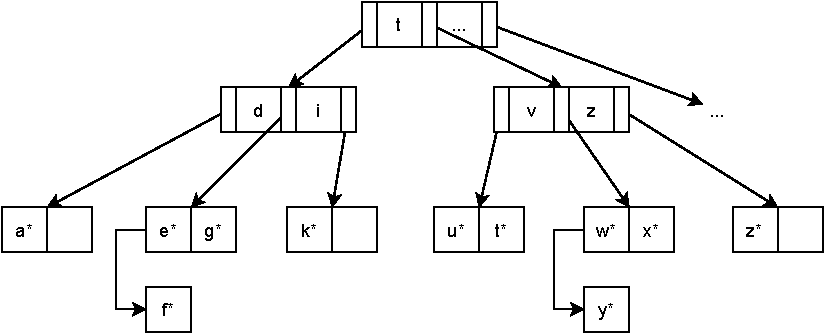
\includegraphics[width=\linewidth]{img/4-1-a-iii.pdf}
        \item 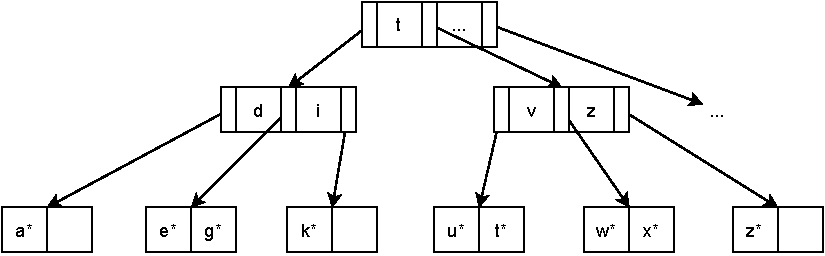
\includegraphics[width=\linewidth]{img/4-1-a-iv.pdf}
    \end{enumerate}

    \item \begin{enumerate}
        \item T
        \item F
        \item F
        \item T
        \item F
    \end{enumerate}
\end{enumerate}

\newpage

\section{B Trees}

\begin{enumerate}
    \item \begin{enumerate}
        \item 12
        \item 11, 22, 33, 44, 55, 66, 77, 88, 99, 110.
    \end{enumerate}

    \item \begin{enumerate}
        \item 1
        \item 6
        \item 31
    \end{enumerate}

    \item 17
\end{enumerate}

\newpage

\section{B+ Trees}

\begin{enumerate}
    \item 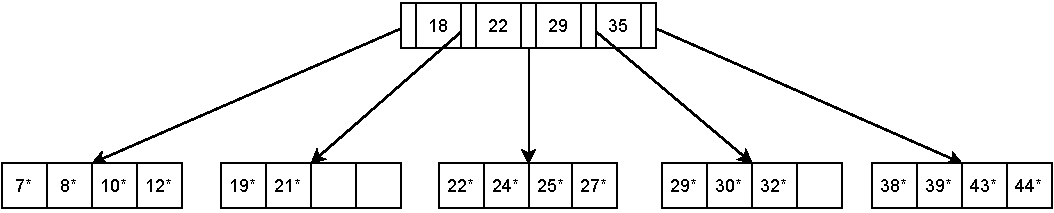
\includegraphics[width=\linewidth]{img/4-3-a.pdf}
    \item 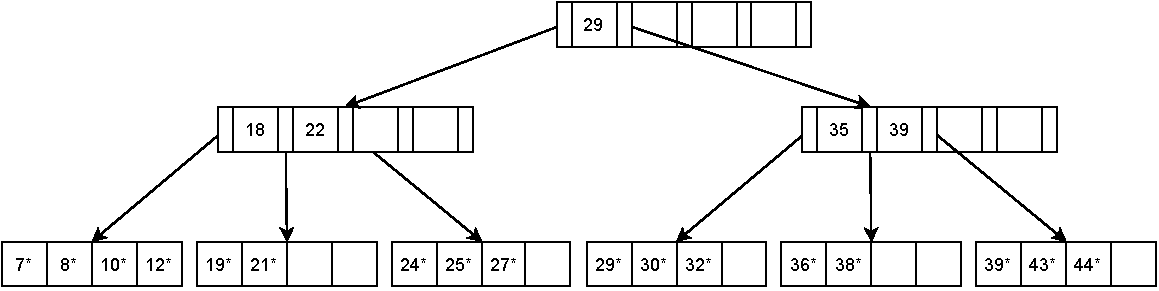
\includegraphics[width=\linewidth]{img/4-3-b.pdf}
    \item 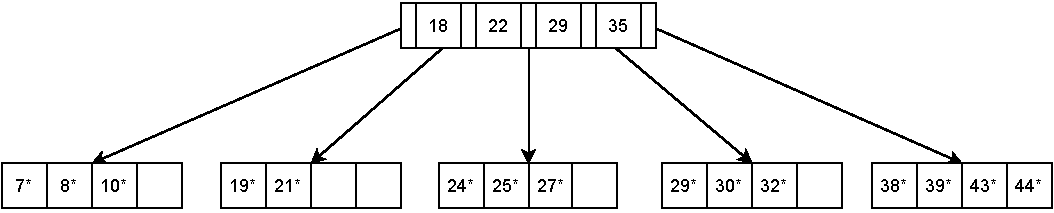
\includegraphics[width=\linewidth]{img/4-3-c.pdf}
    \item 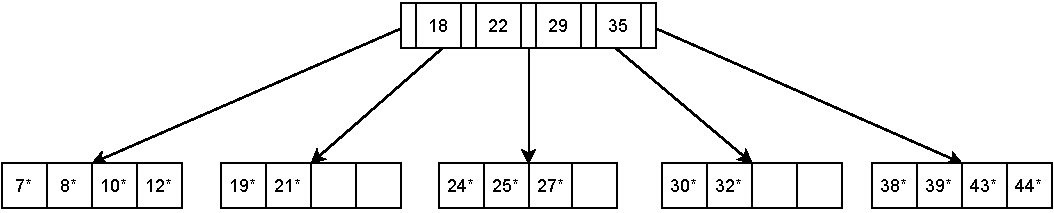
\includegraphics[width=\linewidth]{img/4-3-d.pdf}
    \item 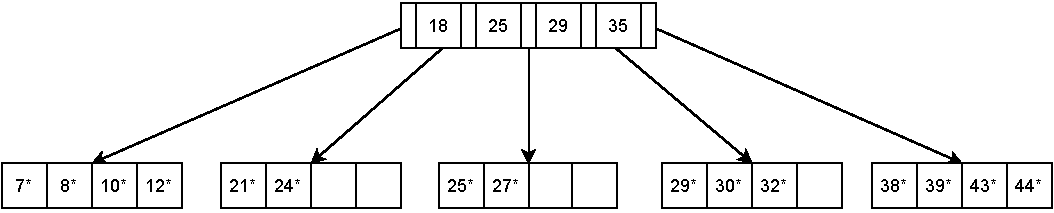
\includegraphics[width=\linewidth]{img/4-3-e.pdf}
\end{enumerate}

\newpage

\section{Extendible Hashing}

\begin{enumerate}
    \item 2
    \item F
    \item \begin{enumerate}
        \item 11
        \item 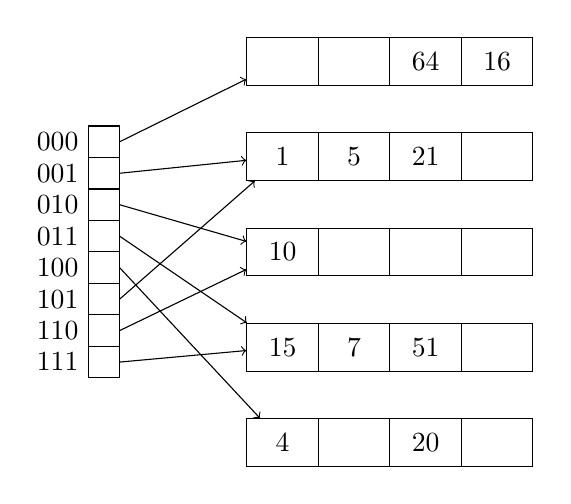
\begin{tikzpicture}[
                bucket/.style={
                    matrix of nodes,
                    ampersand replacement=\&,
                    nodes={
                        draw, anchor=center,
                        minimum width=6ex, minimum height=4ex
                    },
                    column sep=-\pgflinewidth, nodes in empty cells
                }
            ]
            \node (directory) [rectangle split, rectangle split parts=8, draw] at (0, -16ex) {
                \nodepart{one}
                \nodepart{two}
                \nodepart{three}
                \nodepart{four}
                \nodepart{five}
                \nodepart{six}
                \nodepart{seven}
                \nodepart{eight}
            };

            \foreach \i/\cells in {0/\& \& 64 \& 16,1/1 \& 5 \& 21 \&,2/10 \& \& \&,3/15 \& 7 \& 51 \&,4/4 \& \& 20 \&}
                \node (bucket \i) [bucket] at (24ex, -\i*8ex) {\cells\\};

            \foreach \part/\label/\bucket in {one/000/0,two/001/1,three/010/2,four/011/3,five/100/4,six/101/1,seven/110/2,eight/111/3} {
                \node [left] at (directory.\part\space west) {\label};
                \draw [->] (directory.\part\space east) -- (bucket \bucket-1-1);
            }
        \end{tikzpicture}
    \end{enumerate}
\end{enumerate}
\newpage

\section{Linear Hashing}

\begin{enumerate}
    \item F
    \item F
    \item \begin{enumerate}
        \item 4th bucket
        \item 63
        \item \begin{tikzpicture}[
                page/.style={
                    node distance=10ex,
                    matrix of nodes,
                    nodes={
                        draw, anchor=center,
                        minimum width=4ex, minimum height=4ex
                    },
                    column sep=-\pgflinewidth, nodes in empty cells, on grid
                }
            ]
            \foreach \i/\x/\y in {0/00/000,1/01/001,2/10/010,3/11/011,4/00/100,5/01/101} {
                \node (h1 \i) at (0, -\i*10ex) {\y};
                \node (h0 \i) [on grid, right=8ex of h1 \i] {\x};
            }

            \node (h0) [above=of h0 0] {$h_0$};
            \node (h1) [above=of h1 0] {$h_1$};

            \draw ($(h1) + (4ex, 2ex)$) -- ($(h1 5) + (4ex, -6ex)$);
            \draw ($(h0) + (5ex, 2ex)$) -- ($(h0 5) + (5ex, -6ex)$);

            \node (page 0) [page, right=18ex of h0 0] {64 & & & \\};
            \draw ($(page 0-1-4.south east) - 1/2*(\pgflinewidth, 0)$) -- ++(0, -2ex) -- +(-1ex, 0) -- +(1ex, 0);

            \node (page 1) [page, below=of page 0] {9 & 25 & 17 & \\};
            \draw ($(page 1-1-4.south east) - 1/2*(\pgflinewidth, 0)$) -- ++(0, -2ex) -- +(-1ex, 0) -- +(1ex, 0);

            \node (page 2) [page, below=of page 1] {10 & & & \\};
            \draw ($(page 2-1-4.south east) - 1/2*(\pgflinewidth, 0)$) -- ++(0, -2ex) -- +(-1ex, 0) -- +(1ex, 0);

            \node (page 3) [page, below=of page 2] {31 & 15 & 7 & 3 \\};
            \node (page 3-0) [page, right=22ex of page 3] {35 & & & \\};
            \draw [->] ($(page 3-1-4.south east) + 1/2*(0, \pgflinewidth)$) -- ($(page 3-0-1-1.south west) + 1/2*(0, \pgflinewidth)$);
            \draw ($(page 3-0-1-4.south east) - 1/2*(\pgflinewidth, 0)$) -- ++(0, -2ex) -- +(-1ex, 0) -- +(1ex, 0);

            \node (page 4) [page, below=of page 3] {44 & & & \\};
            \draw ($(page 4-1-4.south east) - 1/2*(\pgflinewidth, 0)$) -- ++(0, -2ex) -- +(-1ex, 0) -- +(1ex, 0);

            \node (page 5) [page, below=of page 4] {5 & 21 & & \\};
            \draw ($(page 5-1-4.south east) - 1/2*(\pgflinewidth, 0)$) -- ++(0, -2ex) -- +(-1ex, 0) -- +(1ex, 0);

            \node [above] at (page 2-1-1.north) {$\mathrm{Next} = 2$};
        \end{tikzpicture}
    \end{enumerate}
\end{enumerate}

\end{document}
